\documentclass[12pt]{report}

\usepackage{commands}
\usepackage{jlcode}

\begin{document}

\large

\begin{center}
 Math 586 Finally Project\\
 By Marvyn Bailly (Github: MarvynB)\\
\end{center}

\normalsize

\hrule

%---------------%
%---Problem 1---%
%---------------%

%--status--$

\begin{problem}
    Consider the ODE:
\begin{align*} v'(t) = \frac 1 \epsilon g(v(t)), \quad g(v) = v (\alpha - v) (v-1) - w. \end{align*}

Using the TR-BDF-2 method,

$$U^* = U^n + \frac k 4 (f(U^n) + f(U^*)),\\
U^{n+1} = \frac 1 3 \left( 4 U^* -U^n + k f(U^{n+1})\right),$$

solve this ODE and verify that the method is indeed second-order accurate at $t = 0.1$.  Use $v(0) = 0.3$, $\alpha= 0.5$, $w = 0.1$ and $\epsilon = 0.01$ as your parameters.

Note that you have to solve two nonlinear systems at each time step.  The first one requires you to solve

$$ G_1(u) = 0, \quad G_1(u) = u - U^n - \frac k 4 (f(U^n) + f(u)), \quad G_1'(u) = 1 - \frac k 4 f'(u).$$

The second is given by

$$ G_2(u) = 0, \quad G_2(u) = u - \frac 1 3 \left( 4 U^* -U^n + k f(u)\right), \quad G_2'(u) = 1 - \frac k 3 f'(u).$$

It is highly recommended that your write a function \verb`TRBDF2(U,w,k)` that advances the solution one time step.  This function may take in the \verb`max_iter` and \verb`tol` for Newton's method as well.
\end{problem}

\begin{solution}

    \noindent
    Consider the ODE:
\begin{align*} v'(t) = \frac 1 \epsilon g(v(t)), \quad g(v) = v (\alpha - v) (v-1) - w. \end{align*}
Using the TR-BDF-2 method,
\begin{equation}\label{TR-BDF-2}
    U^* = U^n + \frac k 4 (f(U^n) + f(U^*)),\\
    U^{n+1} = \frac 1 3 \left( 4 U^* -U^n + k f(U^{n+1})\right),
\end{equation}
we wish to solve this ODE and verify that the method is indeed second-order accurate at $t=0.1$. We will use $v(0)=0.3,\alpha=0.5,w=0.1,\and,\eps=0.01$ as the parameters. We will write a function \verb+TRBDF2(U,w,k,max_iter,tol)+ that applies one step of the method to the solution. We implement this function in Julia as following
\begin{jllisting}
function TRBDF2(U,w,k,max_iter,tol)
    function G1(u)
        u - U - k/4 * (f(U) + f(u))
    end
    function G1_prime(u)
        1 - k/4 * f_prime(u)
    end
    function G2(u)
        u - 1/3 * (4*Us - U + k*f(u))
    end
    function G2_prime(u)
        1 - k/3 * f_prime(u)
    end
    function g(u)
        u*(α - u)*(u-1)-w
    end
    
    function f(x)
        (1/ϵ) * g(x)
    end
    
    function f_prime(u)
        (1/ϵ)*(2 * u * α - α - 3*u^2 + 2*u)
    end

    Us = Newton(U,G1,G1_prime,300,1e-10)
    U = Newton(Us,G2,G2_prime,300,1e-10)
end
\end{jllisting}
which depends on the following implementation of Newton's method
\begin{jllisting}
function Newton(U,f,Df,max_iter,tol)
    for j=1:max_iter
        U = U .- f(U)./Df(U)
        if maximum(abs.(f(U))) < tol
            break
        end
    end
    return U
end
\end{jllisting}
Now to see if the method is working, we plot the evolution of the solution using $k=0.001$ from $t=0$ to $t=0.1$ to get the plot shown in Figure \ref{q1-sol} which appears to be demonstrating the correct behavior of the solution. Next, we will numerically show that the method is second-order accurate at $t=0.1$ by creating a reference solution using a small step size of $k=2^{-10}t$. Next, we compute the solution at $t=0.1$ using increasingly small $k$ values, $k=2^(-j)t$ for $j=1,2,\cdots,8$ and computed the maximum absolute error from the reference solution. Plotting the maximum errors along with $y=h^2$ we see the errors decrease with $y=h^2$ as seen in Figure \ref{q1-err}. Therefore we conclude that this method is second-order accurate.  

\begin{figure}
    \centering
    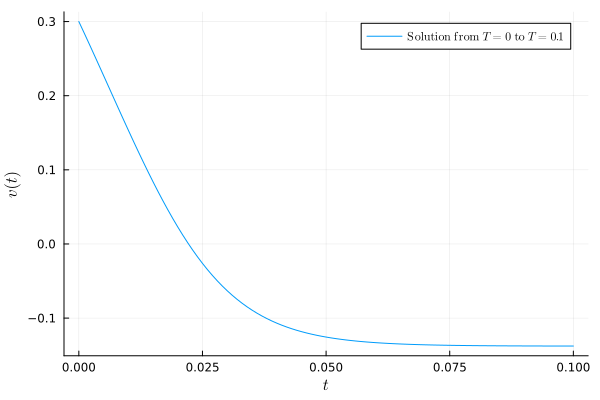
\includegraphics[width=0.75\textwidth,height=\textwidth,keepaspectratio]{images/1-sol.png}
    \caption{Evolution of solution from $t=0$ to $t=0.1$ using $k=0.001$.}
    \label{q1-sol}    
\end{figure} 

\begin{figure}[H]
    \centering
    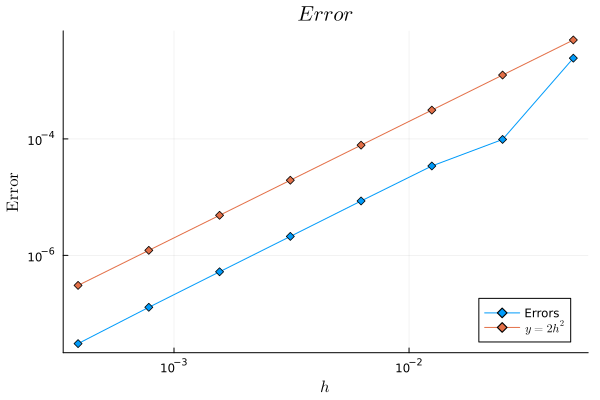
\includegraphics[width=0.75\textwidth,height=\textwidth,keepaspectratio]{images/1-err.png}
    \caption{Maximum errors, seen in blue, between reference solution, $k=T2^{-10}$, and increasingly small $k$ values at $t=0.1$. In red $y=2h^2$.}
    \label{q1-err}
\end{figure}


\end{solution}

%----------------------------------------------------------------------------------------------------%
%\vskip 20pt
\newpage

%---------------%
%---Problem 1---%
%---------------%

%--status--$

\begin{problem}
    The previous ODE becomes more interesting when it is coupled with another differential equation that evolves $w$:
\begin{align*} v'(t) &= \frac 1 \epsilon \left( g(v(t)) - w(t) + I_a \right), \quad g(v) = v (\alpha - v) (v-1),\\
w'(t) &= \beta v(t) - \gamma w(t).\end{align*}
This is a simple model that exhibits many features of excitable media, and is a simplification of the famous Hodgkin-Huxley equations that are a model for propagation in neuronal systems.  In this system $v(t)$ models the membrane potential while $w(t)$ models the concentration of an ion.
Since we have already gone through the effort to solve the above system, we would like to be able to reuse our code.  Write the system as
\begin{align*}
\begin{bmatrix} v'(t) \\ w'(t) \end{bmatrix} = \mathcal A\left(\begin{bmatrix} v(t) \\ w(t) \end{bmatrix} \right) + \mathcal B\left(\begin{bmatrix} v(t) \\ w(t) \end{bmatrix} \right)
\end{align*}
where
\begin{align*}
\mathcal A \left(\begin{bmatrix} v \\ w \end{bmatrix} \right) &= \begin{bmatrix} \frac 1 \epsilon \left( g(v) - w+ I_a \right) \\ 0\end{bmatrix}, \\
\mathcal B \left(\begin{bmatrix} v \\ w \end{bmatrix} \right) &= \begin{bmatrix} 0 \\ \beta v - \gamma w\end{bmatrix}.
\end{align*}
In the notation of (11.24) in the text, the function \verb`TRBDF2(V,W,k)` described in the previous problem is the function $\mathcal N_{\mathcal A}(V,W,k)$.  Construct the analogous function for $\mathcal N_{\mathcal B}(V,W,k)$, call it \verb`RK2(V,W)` using the second-order Runge-Kutta method (5.30).
Then \verb`Julia` code for Strang splitting (11.24) is given by
\begin{jllisting}
W[i] = RK2(V[i-1],W[i-1],k/2)
V[i] = TRBDF2(V[i-1],W[i],k)
W[i] = RK2(V[i],W[i],k/2)
\end{jllisting}
This should be easily adapted to the language of your choosing.
Using
\begin{align*}
\alpha = 0.3, \quad \beta = 1, \quad \gamma = 1, \quad I_a = 0, \quad \epsilon = 0.001,
\end{align*}
with initial data
\begin{align*}
v(0) = v_0, \quad w(0) = 0,
\end{align*}
the solution of the ODE system exhibits two distinct behaviors:

1. If $v_0 = 0.31$ then $v(t)$ rapdily rises near $v = 1$ and then decays to the stable steady state $v = w = 0$.

2. If $v_0 = 0.29$ the the solution decays directly to the steady state $v = w = 0$.
\noindent
Verify the plot these two solutions. Numerically, verify that your method is second-order accurate at $t = 0.25$ when $v_0 = 0.29$.
Lastly, change $I_a = 0.2$ and plot the solution with $v_0 = 0$ until $t = 10$.
\end{problem}

\begin{solution}

    \noindent
    Consider modifying the previous ODE such that it is coupled with another differential equation that evolves $w$:
    \begin{align*} 
        v'(t) &= \frac 1 \epsilon \left( g(v(t)) - w(t) + I_a \right), \quad g(v) = v (\alpha - v) (v-1),\\
        w'(t) &= \beta v(t) - \gamma w(t).
    \end{align*}
    We will rewrite this system as
    \begin{align*}
        \begin{bmatrix} v'(t) \\ w'(t) \end{bmatrix} = \mathcal A\left(\begin{bmatrix} v(t) \\ w(t) \end{bmatrix} \right) + \mathcal B\left(\begin{bmatrix} v(t) \\ w(t) \end{bmatrix} \right)
        \end{align*}
        where
        \begin{align*}
        \mathcal A \left(\begin{bmatrix} v \\ w \end{bmatrix} \right) &= \begin{bmatrix} \frac 1 \epsilon \left( g(v) - w+ I_a \right) \\ 0\end{bmatrix}, \\
        \mathcal B \left(\begin{bmatrix} v \\ w \end{bmatrix} \right) &= \begin{bmatrix} 0 \\ \beta v - \gamma w\end{bmatrix}.
    \end{align*}
    We will use a Strang splitting method to solve this problem by splitting into $\mathcal N_{\mathcal A}(V,W,k)$ and $\mathcal N_{\mathcal B}(V,W,k)$. To solve $\mathcal N_{\mathcal A}(V,W,k)$ we will modify the previous \verb+TRBDF2(U,w,k,max_iter,tol)+ to fit the updated $v'(t)$ function as seen in the following code:
    \begin{jllisting}
function TRBDF2(U,w,k,max_iter,tol)
    function G1(u)
        u .- U .- k/4 .* (f(U) .+ f(u))
    end
    
    function G1_prime(u)
        1 .- k/4 .* f_prime(u)
    end
    
    function G2(u)
        u .- 1/3 .* (4 .* Us .- U .+ k .* f(u))
    end
    
    function G2_prime(u)
        1 .- k/3 .* f_prime(u)
    end
    function g(v)
        v .* (α .- v) .* (v .- 1)
    end
    
    function f(x)
        (1 ./ ϵ) .* (g(x) .- w .+ Ia)
    end
    
    function f_prime(u)
        (1 ./ ϵ) .* (2 .* u .* α .- α .- 3 .* u^2 .+ 2 .* u)
    end
    
    Us = Newton(U,G1,G1_prime,300,1e-10)
    U = Newton(Us,G2,G2_prime,300,1e-10)
end
    \end{jllisting}
    To handle $\mathcal N_{\mathcal B}(V,W,k)$, we will use the second-order Runge-Kutta method and call the function \verb+RK2(V,W)+ which is implemented in the following code: 
    \begin{jllisting}
function RK2(V,W,k)
    function h(W,V)
        β.*V .- γ.*W
    end
    Wtemp = W .+ (k/2) .* h(W,V)
    W = W .+ k .* h(Wtemp,V)
end
    \end{jllisting}
    The Strang splitting method we use is given by
    \begin{jllisting}
W[i] = RK2(V[i-1],W[i-1],k/2)
V[i] = TRBDF2(V[i-1],W[i],k,300,1e-10)
W[i] = RK2(V[i],W[i],k/2)
    \end{jllisting}
    We will use the parameters $\alpha = 0.3, \beta = 1, \gamma = 1, I_a = 0, \and \epsilon = 0.001$ with the initial conditions $v(0) = v_0, \quad w(0) = 0.$ 

    \noindent
    We will first plot the evolution of the solution for $v_0 =0.31$ on $t=0$ to $t=1.5$ which can be seen in Figure \ref{2sol1}. We see that $v(t)$ rapidly rises near $v(t)=1$ and then decays to the stable steady state of $v(t) = w(t) = 0$. We also see that $w(t)$ increases until it intersects $v(t)$ and then decreases to the stable steady state. 
    
    \noindent
    Next, we will plot the evolution of the solution for $v_0 = 0.29$ on the $t=0$ to $t=0.25$ which can be seen in Figure \ref{2sol2}. We see that solution $v(t)$ decays directly to the steady state and once again it appears that $w(t)$ slightly increases until it intersects $v(t)$ and then decreases to the steady state.  

    \noindent
    Next, we will numerically verify that our method is second-order accurate at $t=0.25$ when $v_0 = 0.29$. We will use the same method as 
    described in question 1 by creating a reference solution using a small $k$ value of $k=2^{-16}t$. We will run the solution for increasingly small $k$ values, $k=t2^{-j}$ for $j=1,2,\cdots,8$ and compute the maximum absolute error of $v(t)$ and $w(t)$ compared to the reference solution for $v(t)$ and $w(t)$. Then plotting the maximum of the max error of $v(t)$ and $w(t)$ at each $k$ step along with $y=h^2$, we see that the errors decrease with $y=h^2$ as seen in Figure \ref{q1-err}. Therefore we conclude that this method is second-order accurate.

    \noindent
    Finally, we change $I_a = 0.2$ and $v_0 = 0$ and plot the evolution of the solution from $t=0$ to $t=10$. We see the solution in Figure \ref{2final} where we notice the relationship between $v(t)$ and $w(t)$. As $v(t)$ spikes to around $v(t)=1$, it decreases until it spikes again. At the same time, $w(t)$ increases until it intersects $v(t)$ and decreases until it intersects $v(t)$ where it increases again.


    \begin{figure}[H]
        \centering
        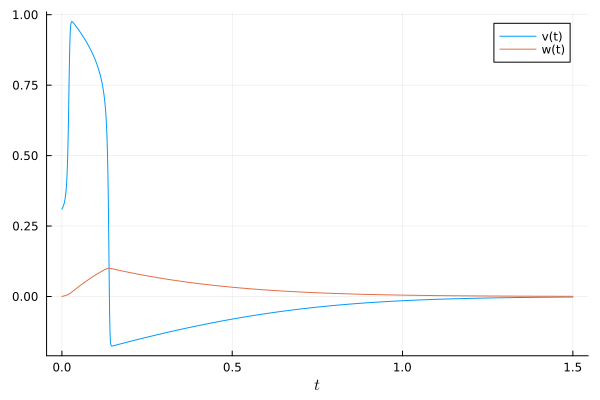
\includegraphics[width=0.75\textwidth,height=\textwidth,keepaspectratio]{images/2-sol1.png}
        \caption{Solution from $t=0$ to $t=1.5$ with $v_0 = 0.31$. $v(t)$ seen in blue while $w(t)$ is seen in orange. }
        \label{2sol1}
    \end{figure}
    \begin{figure}[H]
        \centering
        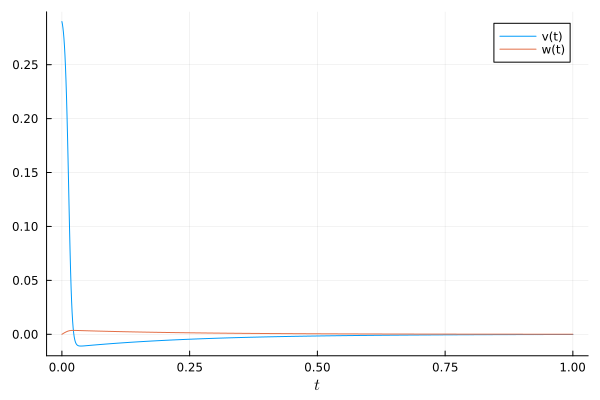
\includegraphics[width=0.75\textwidth,height=\textwidth,keepaspectratio]{images/2-sol2.png}
        \caption{Solution from $t=0$ to $t=1.5$ with $v_0 = 0.29$. $v(t)$ seen in blue while $w(t)$ is seen in orange. }
        \label{2sol2}
    \end{figure}
    \begin{figure}[H]
        \centering
        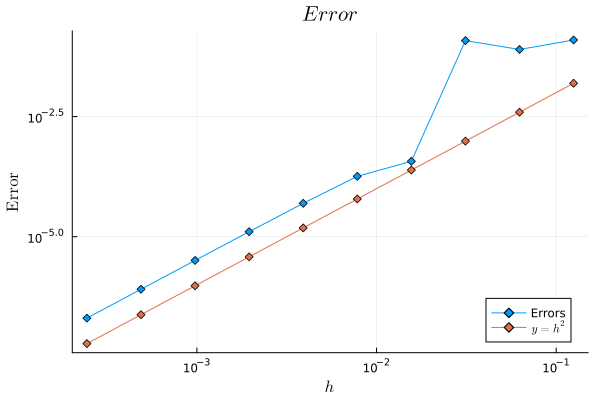
\includegraphics[width=0.75\textwidth,height=\textwidth,keepaspectratio]{images/2-err.png}
        \caption{Plot of the max of the maximum absolute error of $v(t)$ and $w(t)$ compared to the reference solution.}
        \label{2err}
    \end{figure}
    \begin{figure}[H]
        \centering
        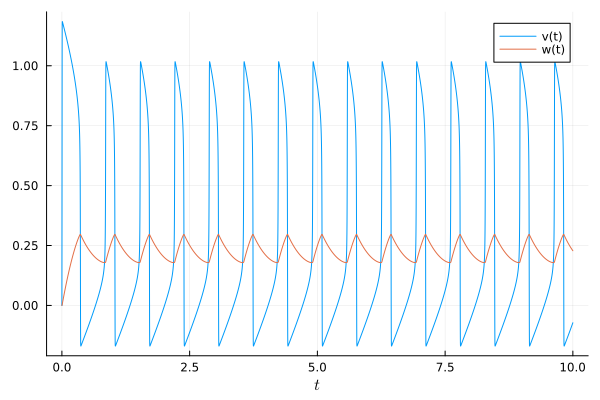
\includegraphics[width=0.75\textwidth,height=\textwidth,keepaspectratio]{images/2-final.png}
        \caption{Solution when $I_a = 0.2$ and $t$ goes from $0$ to $10$.}
        \label{2final}
    \end{figure}







\end{solution}

%----------------------------------------------------------------------------------------------------%
%\vskip 20pt
\newpage

%---------------%
%---Problem 1---%
%---------------%

%--status--$

\begin{problem}
    Consider the heat equation
\begin{align*}
    v_t = \kappa v_{xx}, \quad t > 0,\quad x \in (a,b).
\end{align*}
We impose Neumann boundary conditions $v_x(a,t) = 0 = v_x(b,t)$.  Because the boundary conditions do not directly specify $v(a,t)$ and $v(b,t)$, we need to include their approximations in our vector of unkowns.  The MOL discretization can be written as
\begin{align*}
V'(t) = \frac{\kappa}{h^2} A V(t),
\end{align*}
where
\begin{align*}
V(t) = \begin{bmatrix} V_0(t)\\ V_1(t) \\ \vdots \\ V_{m+1}(t) \end{bmatrix},
\end{align*}
and 
\begin{align*}
A = \begin{bmatrix}
-2  & 2\\
1 & -2 & 1 \\
& 1 & -2 & 1\\
&& \ddots & \ddots & \ddots \\
&&& 1 & -2 & 1\\
&&&& 2 & -2 \end{bmatrix}.
\end{align*}
Note:  This is derived by introducing "ghost values" $V_{-1}(t)$ and $V_{m+2}(t)$ and then enforcing the Neumann conditions via
\begin{align*}
    \frac{V_{1}(t) - V_{-1}(t)}{2h} = 0 = \frac{V_{m+2}(t) - V_{m}(t)}{2h}.
\end{align*}
These relations are used to then eliminate the ghost values from the system.  You need not derive this.  
Apply the TR-BDF-2 method to the MOL discretization and write a function \verb`TRBDF2_heat(V)` that applies one time step of this method with time step \verb`k`.  It is best to keep \verb`k` fixed here because then matrices do not have to be recomputed at each time step.  With $a = 0, b = 4$, demonstrate that your code works by using the initial data
\begin{align*}
    v(x,0) = \begin{cases} 1 &a \leq x < \frac{a+b}{2} \\
    0 & \text{otherwise}.
    \end{cases}
\end{align*}
The integral of the solution should nearly be preserved, resulting in a long-time limit $v(x,t) \approx 1/2$ as $t \to \infty$.  Demonstrate this with $h = 0.01$, $k = h$ and $\kappa = 1$ and discuss any discrepancy you see.  It may help to choose other initial data to explain the situation.
Note: Here you are working on an interval $[a,b]$ and in this case $h$ is affected by the difference $b -a$.
\end{problem}

\begin{solution}
    
    \noindent
    Consider the heat equation
\begin{align*}
    v_t = \kappa v_{xx}, \quad t > 0,\quad x \in (a,b),
\end{align*}
    with Neumann boundary conditions $v_x(a,t) = 0 = v_x(b,t)$.  Because the boundary conditions do not directly specify $v(a,t)$ and $v(b,t)$, we need to include their approximations in our vector of unknowns. The MOL discretization can be written as
    \begin{align*}
    V'(t) = \frac{\kappa}{h^2} A V(t),
    \end{align*}
    where
    \begin{align*}
    V(t) = \begin{bmatrix} V_0(t)\\ V_1(t) \\ \vdots \\ V_{m+1}(t) \end{bmatrix},
    \end{align*}
    and 
    \begin{align*}
    A = \begin{bmatrix}
    -2  & 2\\
    1 & -2 & 1 \\
    & 1 & -2 & 1\\
    && \ddots & \ddots & \ddots \\
    &&& 1 & -2 & 1\\
    &&&& 2 & -2 \end{bmatrix}.
    \end{align*}
    We wish to use our TRBDF-2 method for the MOL discretization and write a function \verb`TRBDF2_heat(V)` that applies one time step of this method. Noticing that we can rewrite \fullref{TR-BDF-2} as 
    \begin{align*}
    \left( I - \frac k 4 A \right)U^*  =  \left( I + \frac k 4 A \right) U^n,\\
    \left( I - \frac k 3 A \right) U^{n+1} = \frac 1 3 \left( 4 U^* - U^n \right),
    \end{align*}
    we implement the \verb`TRBDF_heat(v)`' as
    \begin{jllisting}
function TRBDF2_heat(U,A1,A2,A3)
    Us = A1 \ (A2 * U)
    return A3\ ((4/3) * Us - (1/3) * U)
end
    \end{jllisting}
    where $A_1 = I - \frac{k}{4}A$, $A_2 = I + \frac{k}{4}A$, and $A_3 = I - \frac{k}{3}A$. Note that as per the recommendation, we define this function for a fixed $k$ to avoid the computation of the matrices on each step. We let $a=0, b=4, h=0.01, k = h, \kappa = 1$ and use the initial condition
    \begin{align*}
        \eta(x) = v(x,0) = \begin{cases} 1 &a \leq x < \frac{a+b}{2} \\
        0 & \text{otherwise}.
        \end{cases}
    \end{align*}
    To demonstrate that our method is working correctly, we note that the integral of the solution should nearly be preserved, resulting in a long-time limit $v(x,t) \approx 1/2$ as $t \to \infty$. We create a nice gif in the Notebook (see src/code/3.gif). Plotting the solution with the initial condition at $t=0.1,2,5,10$ we see in Figure \ref{3sol} that the $v(x,t) \approx 1/2$ as $t$ gets big as desired. But if we take a closer look at the solution as $t$ gets large, we see that the solution is settling at a position that is pretty far away from $v(x,t) = 1/2$ as seen in Figure. Computing the maximum error between the solution and $1/2$ we get an error of $0.0012527925659450156$ which is pretty far off from $1/2$ . If we try an initial condition such as
    \[
        \eta_1(x) = \cos\paren{\frac{\pi}{4}x},
    \]
    we expect the method to be able to handle the initial condition since it is a solution to the PDE and expect $v(x,t) \to 0$ as $t \to \infty$. When computing the maximum error between the solution at $t=100$ and $0$ we get an error of $1.807789142202125e-13$. This could show a slight discrepancy in our numerical method. 
    
    \begin{figure}[H]
        \begin{subfigure}[b]{0.45\linewidth}
            \centering
            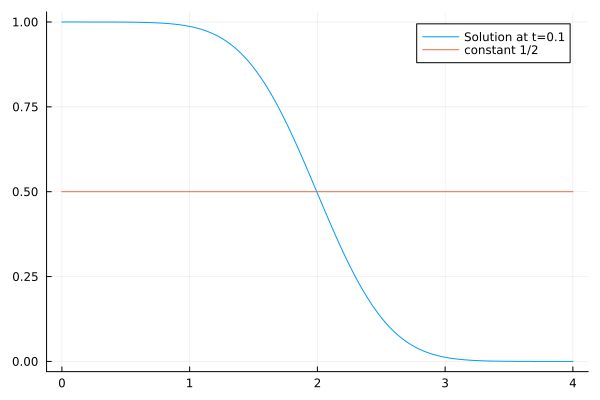
\includegraphics[width=\linewidth]{images/3-1.png}
            \caption{Solution at $t=0.1$.}
            \label{3sol:a}
            \vspace{4ex}
        \end{subfigure}%%
        \begin{subfigure}[b]{0.45\linewidth}
            \centering
            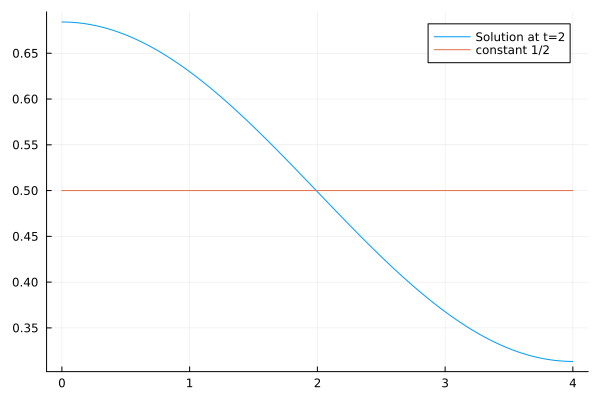
\includegraphics[width=\linewidth]{images/3-2.png}
            \caption{Solution at $t=2.0$.}
            \label{3sol:b}
            \vspace{4ex}
        \end{subfigure}
        \begin{subfigure}[b]{0.45\linewidth}
            \centering
            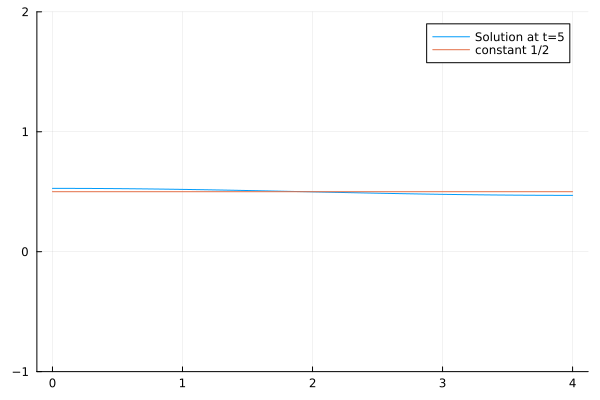
\includegraphics[width=\linewidth]{images/3-3.png}
            \caption{Solution at $t=5.0$.}
            \label{3sol:c}
            \vspace{4ex}
        \end{subfigure}
        \begin{subfigure}[b]{0.45\linewidth}
            \centering
            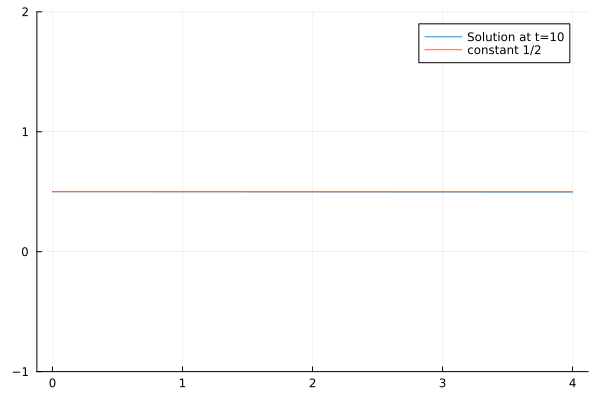
\includegraphics[width=\linewidth]{images/3-4.png}
            \caption{Solution at $t=10.0$.}
            \label{3sol:d}
            \vspace{4ex}
        \end{subfigure}
        \begin{subfigure}[b]{0.45\linewidth}
            \centering
            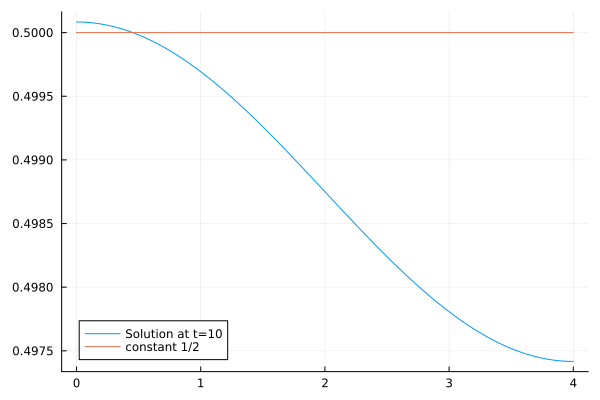
\includegraphics[width=\linewidth]{images/3-5.png}
            \caption{A closer look at solution at $t=10.0$.}
            \label{3sol:e}
            \vspace{4ex}
        \end{subfigure}
        \begin{subfigure}[b]{0.45\linewidth}
            \centering
            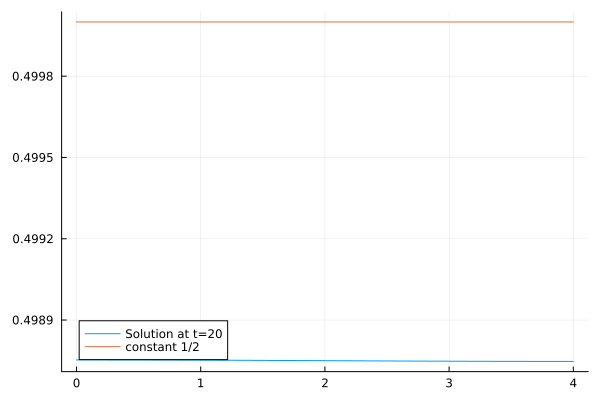
\includegraphics[width=\linewidth]{images/3-6.png}
            \caption{Solution at $t=20.0$.}
            \label{3sol:f}
            \vspace{4ex}
        \end{subfigure}
        \caption{Solution using the initial condition $\eta(x)$ at $t=0.1,2.0,5.0,10.0, \and 20.0$. The solution is shown in blue while a constant $v=1/2$ is shown in orange.}
        \label{3sol}
    \end{figure}
\end{solution}



%----------------------------------------------------------------------------------------------------%
%\vskip 20pt
\newpage

%---------------%
%---Problem 1---%
%---------------%

%--status--$

\begin{problem}
    The ODE system can be modified to allow for spatial variations: For $x \in (a,b)$
\begin{align*}
v_t(x,t) &= \kappa v_{xx}(x,t)+  \frac 1 \epsilon \left( g(v(x,t)) - w(x,t) + I_a \right), \quad g(v) = v (\alpha - v) (v-1),\\
w_t(x,t) &= \beta v(x,t) - \gamma w(x,t)\\
v_x(a,t) & = 0,\\
v_x(b,t) & = 0.
\end{align*}
Now let function \verb`TRBDF2_heat(V)` apply one time step toward the solution of $v_t = \kappa v_{xx}$ with time step \verb`k/2`. Supposing that our previous code for \verb`TRBDF2()` and \verb`RK2()` is vectorized, Strang splitting becomes (with $I_a = 0$)
\begin{jllisting}
    V = TRBDF2_heat(V)
    W = RK2(V,W,k/2)
    V = TRBDF2(V,W,k)
    W = RK2(V,W,k/2)
    V = TRBDF2_heat(V)
\end{jllisting}
Use the parameters:
\begin{align*}
h = 0.02, \quad k = h/10, \quad a = 0, \quad b = 6, \quad \alpha = 0.3,\\
\beta = 1, \quad \gamma = 1, \quad \kappa = 0.2, \quad \epsilon = 0.001.
\end{align*}
and initial data
\begin{align*}
    v(x,0) = \begin{cases} 1 &0 \leq x < 1 \\
    0 & \text{otherwise},
    \end{cases} \quad w(x,0) = 0.
\end{align*}
Solve until $t = 4$.  You should see a travelling wave develop and propagate.
\end{problem}

\begin{solution}
    \noindent
    Consider the modified ODE system which allows for spatial variations: For $x \in (a,b)$
\begin{align*}
v_t(x,t) &= \kappa v_{xx}(x,t)+  \frac 1 \epsilon \left( g(v(x,t)) - w(x,t) + I_a \right), \quad g(v) = v (\alpha - v) (v-1),\\
w_t(x,t) &= \beta v(x,t) - \gamma w(x,t)\\
v_x(a,t) & = 0,\\
v_x(b,t) & = 0.
\end{align*}
We will let the function \verb`TRBDF2_heat(V)` apply one-time step toward the solution of $v_t = \kappa v_{xx}$ with time step \verb`k/2`. To account for the new time step, we modify the matrices $A_1,A_2,\and A_3$ to $A_1 = I - \frac{k}{8}A$, $A_2 = I + \frac{k}{8}A$, and $A_3 = I - \frac{k}{6}A$ to account for the half time step. Now using our previous code for \verb`TRBDF2()` and \verb`RK2()`, we apply the Strang splitting (with $I_a = 0$) of the form
\begin{jllisting}
function solve_strange(V,W,T)
    n = convert(Int64,ceil(T/k))  
    t=0
    n = convert(Int64,ceil(T/k))  
    for i = 2:n+1
        t += k
        #STRANG SPLITTING
        V = TRBDF2_heat(V) #V=0
        W = RK2(V,W,k/2)
        V = TRBDF2(V,W,k,300,1e-10) #V,W
        W = RK2(V,W,k/2)
        V = TRBDF2_heat(V)
    end
    return V,W
end
\end{jllisting}
Now using the parameters:
\begin{align*}
h = 0.02, \quad k = h/10, \quad a = 0, \quad b = 6, \quad \alpha = 0.3,\\
\beta = 1, \quad \gamma = 1, \quad \kappa = 0.2, \quad \epsilon = 0.001,
\end{align*}
and initial data
\begin{align*}
    v(x,0) = \begin{cases} 1 &0 \leq x < 1 \\
    0 & \text{otherwise},
    \end{cases} \quad w(x,0) = 0,
\end{align*}
we solve the modified ODE system until $t = 4$. In my Jupiter notebook, we create a nice gif (see /src/code/4.gif) of the evolution of the solutions $v(x,t)$ and $w(x,t)$ from $t=0$ to $t=4$. In the gif and the four presented figures in Figure \ref{4sol}, we see a traveling wave emerge at $t=0$ and travel to the right as time increases. It is super neat to see how the same interaction between $v(x,t)$ and $w(x,t)$ as discussed in the previous questions is present and appears to drive the traveling wave.   


\begin{figure}[H]
    \begin{subfigure}[b]{0.45\linewidth}
        \centering
        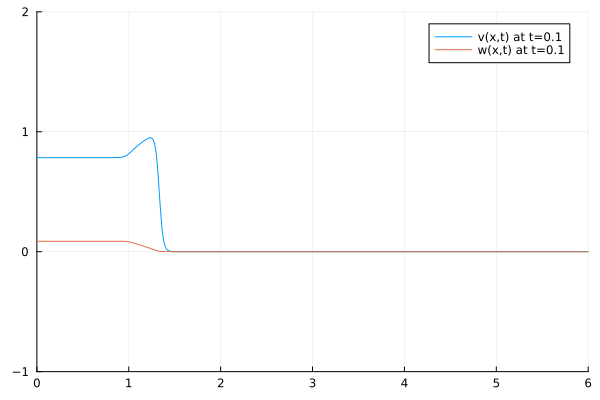
\includegraphics[width=\linewidth]{images/4-1.png}
        \caption{Solution at $t=0.1$.}
        \label{4sol:a}
        \vspace{4ex}
    \end{subfigure}%%
    \begin{subfigure}[b]{0.45\linewidth}
        \centering
        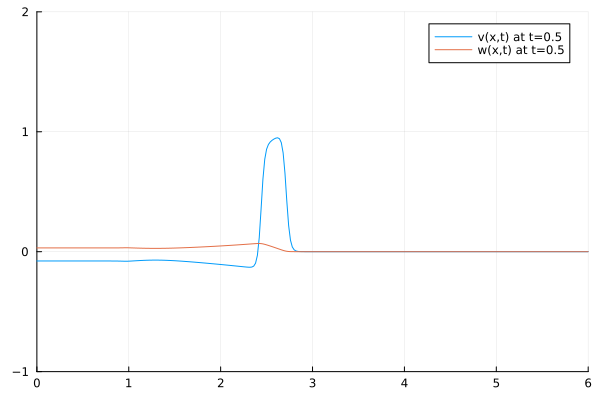
\includegraphics[width=\linewidth]{images/4-2.png}
        \caption{Solution at $t=0.5$.}
        \label{4sol:b}
        \vspace{4ex}
    \end{subfigure}
    \begin{subfigure}[b]{0.45\linewidth}
        \centering
        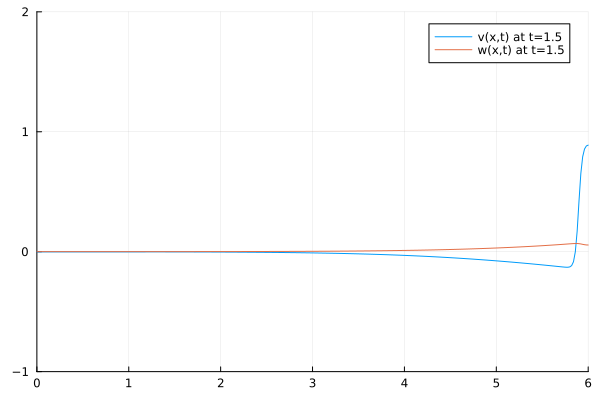
\includegraphics[width=\linewidth]{images/4-3.png}
        \caption{Solution at $t=1.5$.}
        \label{4sol:c}
        \vspace{4ex}
    \end{subfigure}%%
    \begin{subfigure}[b]{0.45\linewidth}
        \centering
        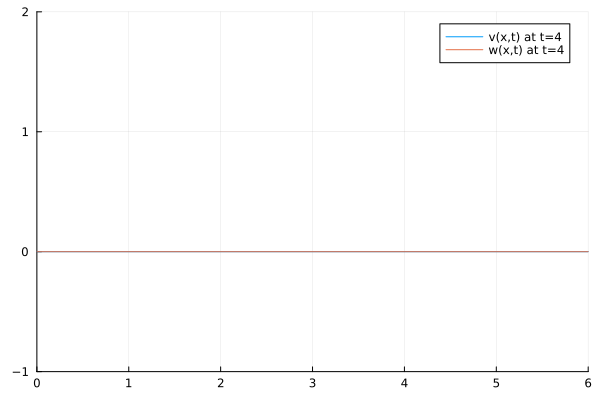
\includegraphics[width=\linewidth]{images/4-4.png}
        \caption{Solution at $t=4.0$.}
        \label{4sol:d}
        \vspace{4ex}
    \end{subfigure}
    \caption{Solutions of the modified system of ODEs. We see $v(x,t)$ in blue and $w(x,t)$ in orange at times $t=0.1,0.5,1.5,\and 4.0$}
    \label{4sol}
\end{figure}

\end{solution}

%----------------------------------------------------------------------------------------------------%
%\vskip 20pt
\newpage

%---------------%
%---Problem 1---%
%---------------%

%--status--$

\begin{problem}
    Repeat the previous problem with

\begin{align*}
    v(x,0) = 0, \quad w(x,0) = 0, \quad I_a(x) = 0.8 e^{-5x^2}.
\end{align*}

This should be a straightforward modification of the code if you've followed the outlined setup and will produce a periodic firing of traveling waves.
\end{problem}

\begin{solution}

    \noindent
    We repeat the previous problem now using
    \begin{align*}
        v(x,0) = 0, \quad w(x,0) = 0, \quad I_a(x) = 0.8 e^{-5x^2}.
    \end{align*}
    We didn't have to make any modifications to our method code. We make a nice gif (see src/code/5.gif)in the notebook which shows a periodic firing of traveling waves. Here we present the solutions at $t=0.1,0.5,1.0,\and 1.5$ in Figure \ref{5sol} which shows waves being periodically created and traveling to the right as time evolves.
    \begin{figure}[H]
        \begin{subfigure}[b]{0.45\linewidth}
            \centering
            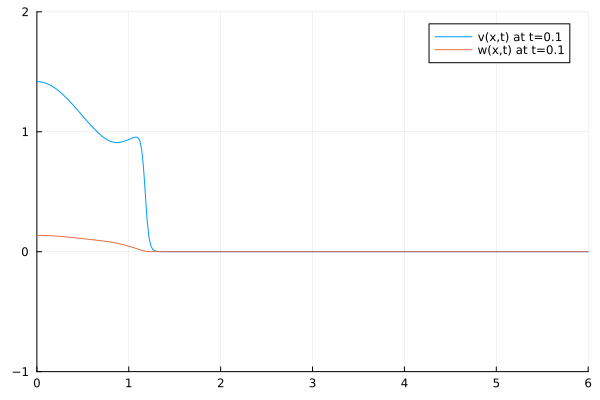
\includegraphics[width=\linewidth]{images/5-1.png}
            \caption{Solution at $t=0.1$.}
            \label{5sol:a}
            \vspace{4ex}
        \end{subfigure}%%
        \begin{subfigure}[b]{0.45\linewidth}
            \centering
            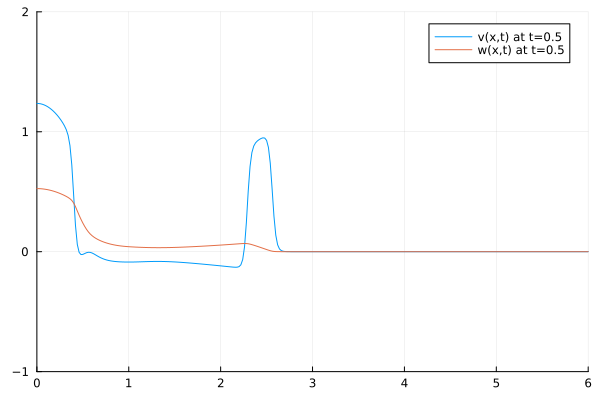
\includegraphics[width=\linewidth]{images/5-2.png}
            \caption{Solution at $t=0.5$.}
            \label{5sol:b}
            \vspace{4ex}
        \end{subfigure}
        \begin{subfigure}[b]{0.45\linewidth}
            \centering
            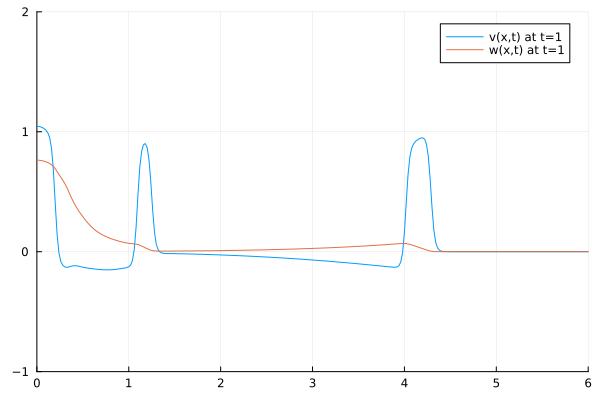
\includegraphics[width=\linewidth]{images/5-3.png}
            \caption{Solution at $t=1.0$.}
            \label{5sol:c}
            \vspace{4ex}
        \end{subfigure}%%
        \begin{subfigure}[b]{0.45\linewidth}
            \centering
            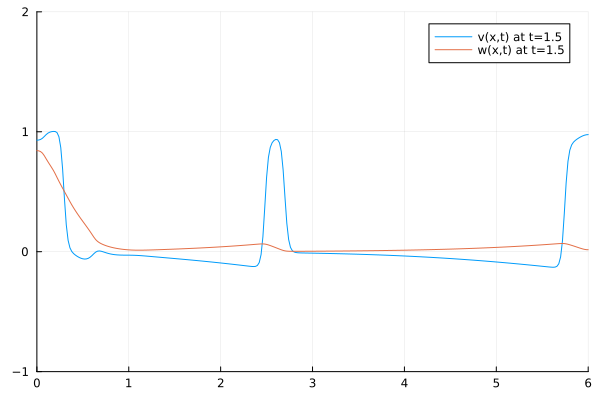
\includegraphics[width=\linewidth]{images/5-4.png}
            \caption{Solution at $t=1.5$.}
            \label{5sol:d}
            \vspace{4ex}
        \end{subfigure}
        \caption{Solutions of the modified system of ODEs. We see $v(x,t)$ in blue and $w(x,t)$ in orange at times $t=0.1,0.5,1.0,\and 1.5$}
        \label{5sol}
    \end{figure}
\end{solution}

%----------------------------------------------------------------------------------------------------%
%\vskip 20pt
\newpage

%---------------%
%---Problem 1---%
%---------------%

%--status--$

\begin{problem}
    Consider the extension of the previous problem to two spatial dimensions: For $x \in (a,b), ~y \in (a,b)$:
\begin{align*}
v_t(x,y,t) &= \kappa v_{xx}(x,y,t) + \kappa v_{yy}(x,y,t)+  \frac 1 \epsilon \left( g(v(x,y,t)) - w(x,y,t) + I_a \right), \quad g(v) = v (\alpha - v) (v-1),\\
w_t(x,y,t) &= \beta v(x,y,t) - \gamma w(x,y,t).
\end{align*}
with initial and boundary data given by
\begin{align*}
v(x,y,0) = \eta(x,y) = \begin{cases} 1 & x < 2,\\
0 & \text{otherwise}, \end{cases} \quad w(x,y,0) = 0,\\
v_x(a,y,t) = v_x(b,y,t) = v_y(x,a,t) = v_y(x,b,t) = 0.
\end{align*}
The code we have created actually immediately generalizes to solve this problem.  Suppose that matrices \verb`W` and \verb`V` contain the spatial array of the values obeying the ordering in Figure 3.2(a).  For example, supposing that the grid spacing is the same in both directions the following code initializes \verb`W` and \verb`V`
\begin{jllisting}
    x = a:h:b |> Array
    y = x
    X = repeat(reshape(x, 1, :), length(y), 1)
    Y = repeat(reverse(y), 1, length(x));
    η = (x,y) -> x < 2 ? 1.0 : 0.0
    V = map(η,X,Y)
    W = 0*V
\end{jllisting}
Then the Strang splitting scheme is given by
\begin{jllisting}
    V = TRBDF2_heat(V)
    V = TRBDF2_heat(V')' |> Array
    W = RK2(V,W,k/2)
    V = TRBDF2(V,W,k)
    W = RK2(V,W,k/2)
    V = TRBDF2_heat(V)
    V = TRBDF2_heat(V')' |> Array
\end{jllisting}
The \verb`|> Array` call just converts the transpose to a real array.  \verb`Julia` has a special data type for the transpose of an array that allows for efficient memory usage but we will avoid using that here.  In \verb`Matlab` or \verb`Python` you wouldn't need an analogous call.
Set the parameters of the problem to be:
\begin{align*}
 a &= 0, \quad b = 12, \quad h = .05, \quad k = h/10, \quad \kappa = 1, \quad \epsilon = 0.01,\\
 \alpha &= 0.1, \quad \beta = 0.5, \quad \gamma = 1, \quad I_a = 0.
 \end{align*}
If you just solve with these parameters you should see a single pulse travel across the domain in the positive $x$-direction. But if at time $t = 0.9$ zero out all elements of $V$ with associated $y$ coordinates being larger than $6$, you break the symmetry in the $y$-direction.  Solve until $t = 6$.  You should see a spiral wave develop! 
\end{problem}

\begin{solution}

    \noindent
    Consider the extension of the previous problem to two spatial dimensions: For $x \in (a,b), ~y \in (a,b)$:
    \begin{align*}
    v_t(x,y,t) &= \kappa v_{xx}(x,y,t) + \kappa v_{yy}(x,y,t)+  \frac 1 \epsilon \left( g(v(x,y,t)) - w(x,y,t) + I_a \right), \quad g(v) = v (\alpha - v) (v-1),\\
    w_t(x,y,t) &= \beta v(x,y,t) - \gamma w(x,y,t).
    \end{align*}
    with initial and boundary data given by
    \begin{align*}
    v(x,y,0) = \eta(x,y) = \begin{cases} 1 & x < 2,\\
    0 & \text{otherwise}, \end{cases} \quad w(x,y,0) = 0,\\
    v_x(a,y,t) = v_x(b,y,t) = v_y(x,a,t) = v_y(x,b,t) = 0.
    \end{align*}
    The code we have created immediately generalizes to solve this problem. We initializes \verb`W` and \verb`V` as
\begin{jllisting}
x = a:h:b |> Array
y = x
X = repeat(reshape(x, 1, :), length(y), 1)
Y = repeat(reverse(y), 1, length(x));
η = (x,y) -> x < 2 ? 1.0 : 0.0
V = map(η,X,Y)
W = 0*V
\end{jllisting}
Then the Strang splitting scheme is given by
\begin{jllisting}
V = TRBDF2_heat(V)
V = TRBDF2_heat(V')' |> Array
W = RK2(V,W,k/2)
V = TRBDF2(V,W,k)
W = RK2(V,W,k/2)
V = TRBDF2_heat(V)
V = TRBDF2_heat(V')' |> Array
\end{jllisting}
We set the parameters of the problem to be:
\begin{align*}
a &= 0, \quad b = 12, \quad h = .05, \quad k = h/10, \quad \kappa = 1, \quad \epsilon = 0.01,\\ \alpha &= 0.1, \quad \beta = 0.5, \quad \gamma = 1, \quad I_a = 0.
\end{align*}
Now running our method, we see a single pulse travel across the domain in the positive $x$ direction. We create a nice gif (see /src/code/6-1.gif) in the Notebook and here we show the solution $v(x,y,t)$ at times $t=0.1,0.6,1.5,\and 1.9$. But now at $t=0.9$, we zero out all the elements corresponding to $y$ coordinates larger than $6$, and we break the symmetry in the $y$-direction resulting in a spiral wave! We implement the interference with
\begin{jllisting}
if t ≈ 0.9
    ind = floor((m + 2) / 2) |> Int
    V[1:ind, :] = zeros(ind, m + 2)
end
\end{jllisting}
We create a nice gif in the Notebook (see /src/code/6-2.gif) but here we show the results at times $t=0.9,2,3,4,5,\and 6$ which shows the spiraling behavior.



\begin{figure}[H]
    \begin{subfigure}[b]{0.45\linewidth}
        \centering
        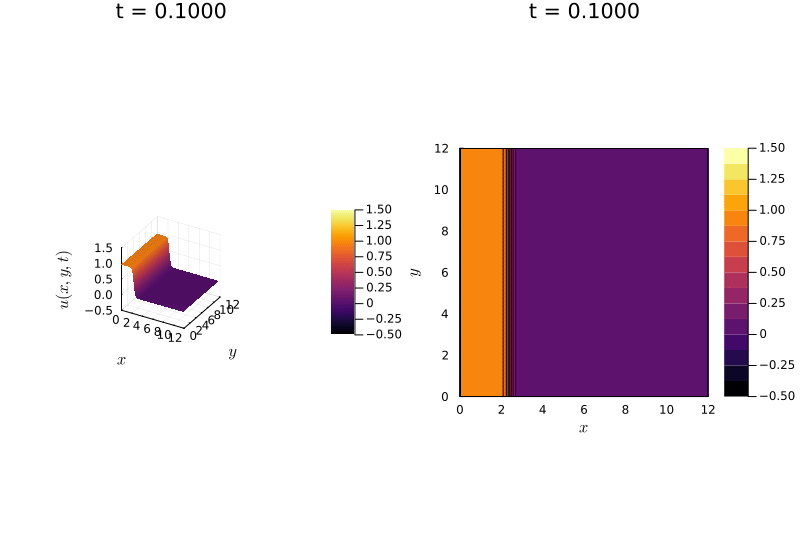
\includegraphics[width=\linewidth]{images/6-1-10.png}
        \caption{Solution at $v(x,y,t)$ at $t=0.1$.}
        \label{6-1:a}
        \vspace{4ex}
    \end{subfigure}%%
    \begin{subfigure}[b]{0.45\linewidth}
        \centering
        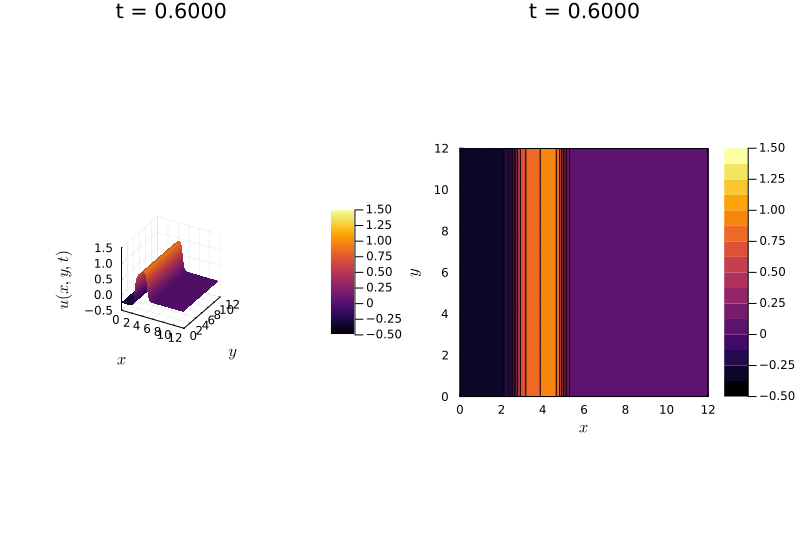
\includegraphics[width=\linewidth]{images/6-1-60.png}
        \caption{Solution at $v(x,y,t)$ at $t=0.6$.}
        \label{6-1:b}
        \vspace{4ex}
    \end{subfigure}
    \begin{subfigure}[b]{0.45\linewidth}
        \centering
        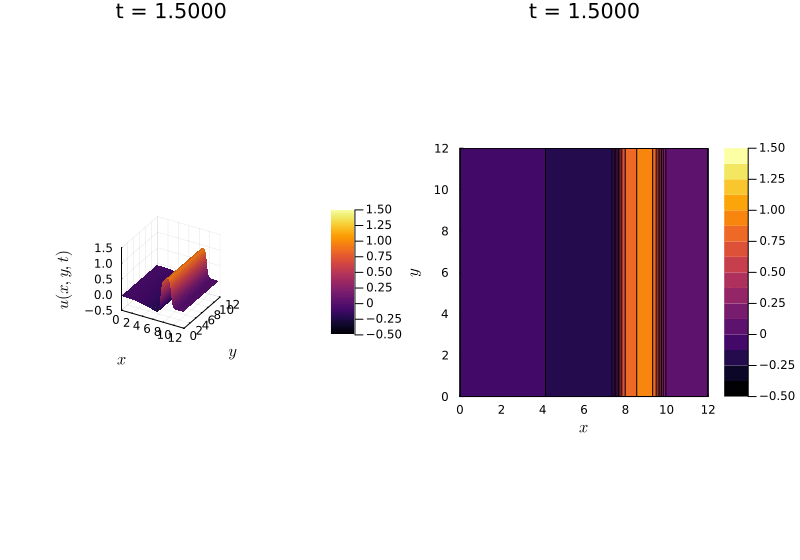
\includegraphics[width=\linewidth]{images/6-1-150.png}
        \caption{Solution at $v(x,y,t)$ at $t=1.5$.}
        \label{6-1:c}
        \vspace{4ex}
    \end{subfigure}%%
    \begin{subfigure}[b]{0.45\linewidth}
        \centering
        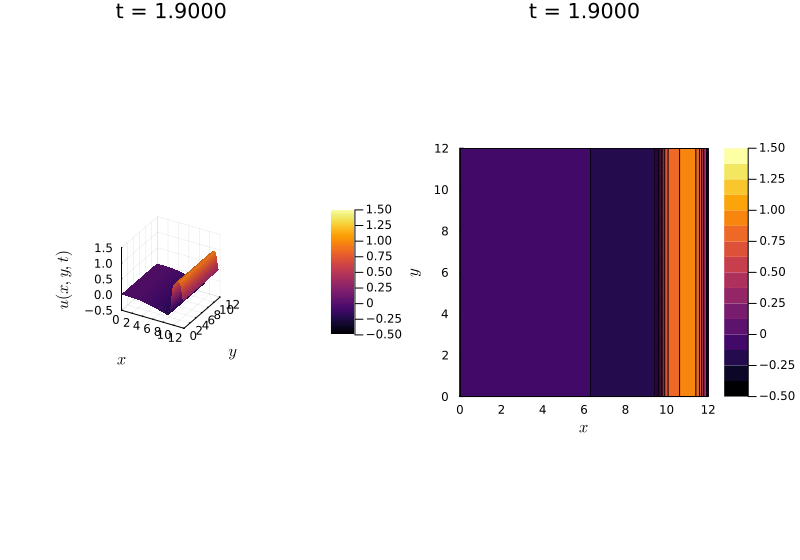
\includegraphics[width=\linewidth]{images/6-1-190.png}
        \caption{Solution at $v(x,y,t)$ at $t=1.9$.}
        \label{6-1:d}
        \vspace{4ex}
    \end{subfigure}
    \caption{Solution $v(x,y,t)$ without interference at $t=0.1,0.6,1.5,\and 1.9$. }
    \label{6-1}
\end{figure}

\begin{figure}[H]
    \begin{subfigure}[b]{0.45\linewidth}
        \centering
        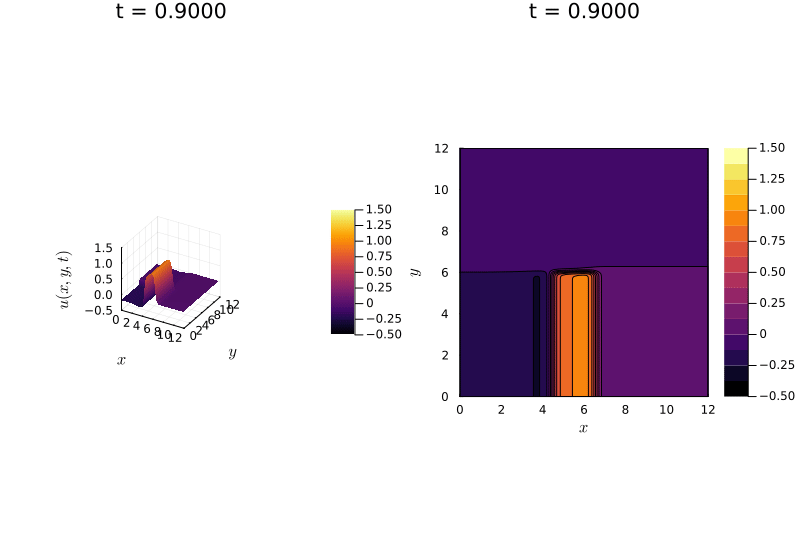
\includegraphics[width=\linewidth]{images/6-2-90.png}
        \caption{Solution at $v(x,y,t)$ at $t=0.9$.}
        \label{6-2:a}
        \vspace{4ex}
    \end{subfigure}%%
    \begin{subfigure}[b]{0.45\linewidth}
        \centering
        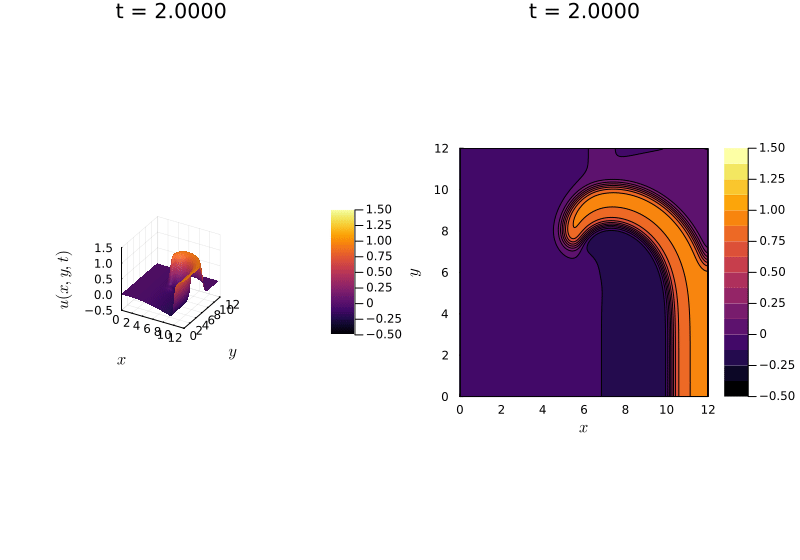
\includegraphics[width=\linewidth]{images/6-2-200.png}
        \caption{Solution at $v(x,y,t)$ at $t=2.0$.}
        \label{6-2:b}
        \vspace{4ex}
    \end{subfigure}
    \begin{subfigure}[b]{0.45\linewidth}
        \centering
        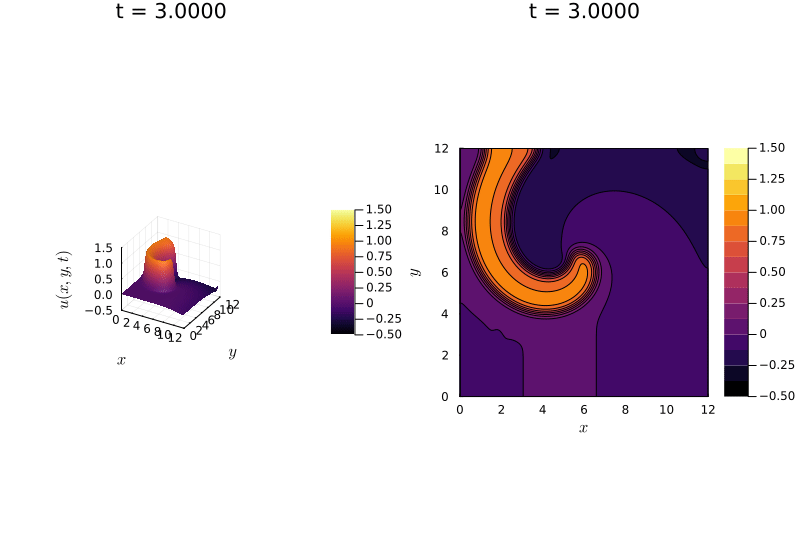
\includegraphics[width=\linewidth]{images/6-2-300.png}
        \caption{Solution at $v(x,y,t)$ at $t=3.0$.}
        \label{6-2:c}
        \vspace{4ex}
    \end{subfigure}%%
    \begin{subfigure}[b]{0.45\linewidth}
        \centering
        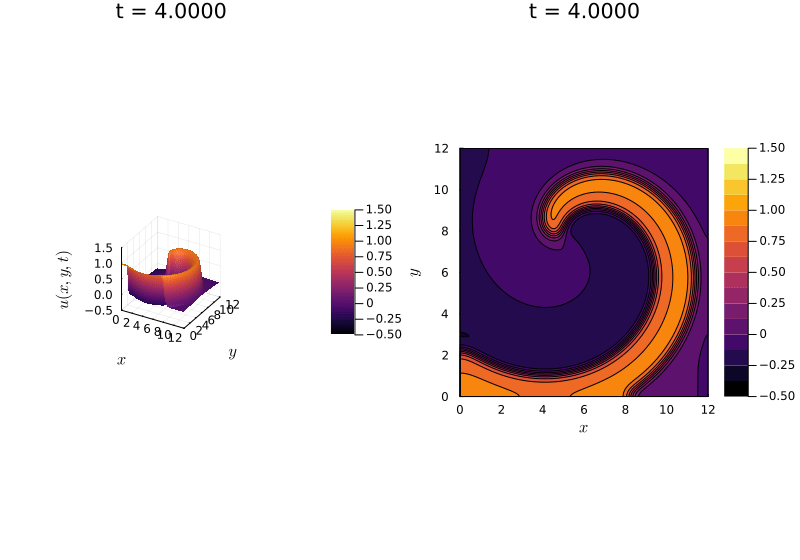
\includegraphics[width=\linewidth]{images/6-2-400.png}
        \caption{Solution at $v(x,y,t)$ at $t=4.0$.}
        \label{6-2:d}
        \vspace{4ex}
    \end{subfigure}
    \begin{subfigure}[b]{0.45\linewidth}
        \centering
        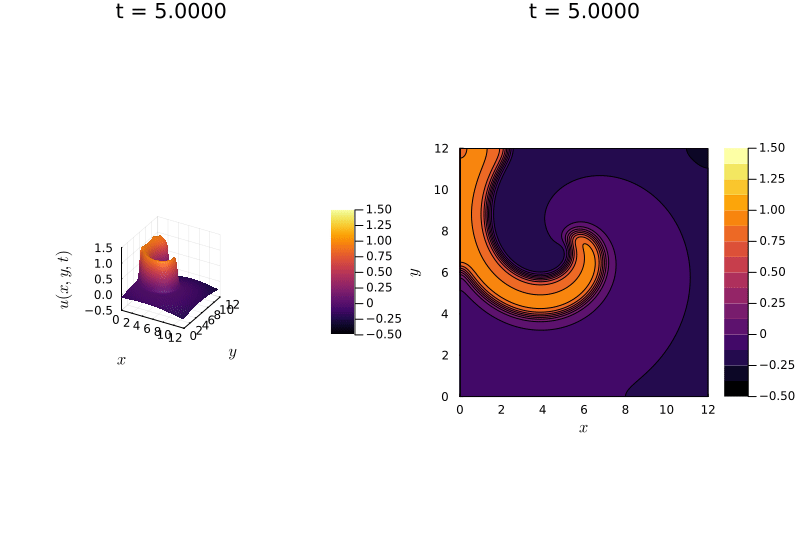
\includegraphics[width=\linewidth]{images/6-2-500.png}
        \caption{Solution at $v(x,y,t)$ at $t=5.0$.}
        \label{6-2:e}
        \vspace{4ex}
    \end{subfigure}%%
    \begin{subfigure}[b]{0.45\linewidth}
        \centering
        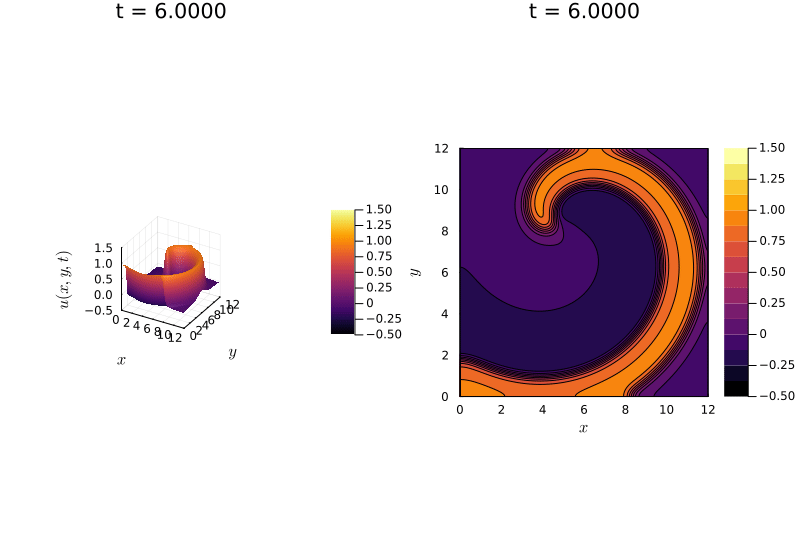
\includegraphics[width=\linewidth]{images/6-2-600.png}
        \caption{Solution at $v(x,y,t)$ at $t=6.0$.}
        \label{6-2:f}
        \vspace{4ex}
    \end{subfigure}
    \caption{Solution $v(x,y,t)$ interference at $t=0.9,2,3,4,5,\and 6$. }
    \label{6-2}
\end{figure}

\end{solution}

%----------------------------------------------------------------------------------------------------%
%\vskip 20pt
\newpage

\end{document}